\begin{figure}
  \centering
  \captionsetup{justification=centering}
  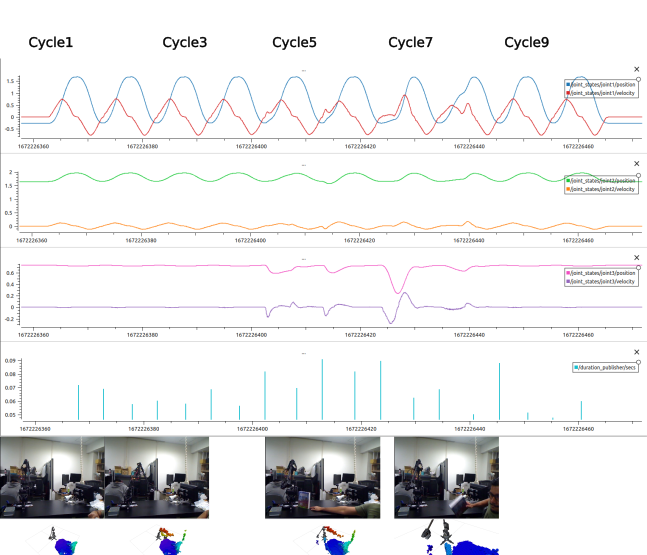
\includegraphics[width=\linewidth]{\thesisDir/chapter5/figures/joints_profiles_with_snapshots_prm.png}
  \caption{The angular displacement and angular velocity for joint1, joint2, joint3, are shown with the planner process time represented by the stick plot. The inset pictures shows the snapshot of the experimentation. The timestamp are represented by the Unix Epoch time format.} 
  \label{fig:joints_profiles_with_snapshots_prm}
\end{figure}

